\documentclass{article}
\usepackage{amsmath}
\usepackage{amssymb}
\usepackage{amsfonts}
\usepackage{mathtools}
\usepackage{mathrsfs}
\usepackage{amsthm}
\usepackage{bbm}
\usepackage{graphicx}
\usepackage{pgfplots}
\usepackage{tikz}

\title{Differential Equations - MATH246}
\author{Tom Mitchell}
\date{Conway - Fall 2024}

\begin{document}

\maketitle

\section*{Class Information}

\subsection*{Grading}
\begin{itemize}
    \item Matlab assignments — 18\% (6\% each)
    \item Quizzes (drop two lowest) — 17\%
    \item Two best in-class exams — 17\% each
    \item Worst in-class exam — 8\%
    \item Final exam — 23\%
\end{itemize}

\subsection*{Office Hours}
\begin{itemize}
    \item Monday: 2:00 PM - 3:00 PM (in person, Kirwin 2400)
    \item Tuesday: 1:15 PM - 2:30 PM (in person, Kirwin 2400)
    \item TBA: Zoom (online)
\end{itemize}

\subsection*{Exams}
\begin{itemize}
    \item 3 midterms and a final exam
\end{itemize}

\section*{Lecture 1, Tuesday 8/27/2024}

\section*{Course Overview: (Differential Equations)}

\section*{Chapter 0:}

A differential equation is an algebraic relation between functions, their derivatives, and independent variables.

\pagebreak

\textbf{Examples:}
\begin{itemize}
    \item \( \left(\frac{dx}{dt}\right)^2 + x \sin(t) = \cos(x) \) \hfill \textit{(Order = 1)}
    \item \( y'' + ty' + y = \cos(t) \) \hfill (Note: \(y' = \frac{dy}{dt})\)\textit{(Order = 2)}
    \item \( \frac{dy}{dt} \cdot \frac{dy}{ds} + y \frac{dz}{dt} = \sin(st) \) \hfill \textit{(Order = 1)}
\end{itemize}

\textbf{Order:} The order of a differential equation is the order of the highest derivative that appears.

\textbf{Notation:} For \( \frac{dy}{dx} \), we can write \( y' \) or \( \dot{y} \) (dot notation).

An ordinary differential equation (ODE) involves no partial derivatives, as opposed to a partial differential equation (PDE).

\textbf{Note:} This course only deals with ODEs.

\subsection*{Linearity of ODEs}

An ODE with function \( y \) and independent variable \( t \) is \textbf{linear} if it can be written as:

\[
a_n(t)y^{(n)} + a_{n-1}(t)y^{(n-1)} + \dots + a_1(t)y' + a_0(t)y = f(t)
\]

\textit{where \( y^{(n)} \) is the \( n \)th derivative of \( y \).}

\textbf{Examples:}
\begin{itemize}
    \item \( \left(\frac{dx}{dt}\right)^2 + x \sin(t) = \cos(x) \) \hfill \textit{(Not linear: \( \left(\frac{dx}{dt}\right)^2 \) and \( \cos(x) \))}
    \item \( y'' + ty' + y = \cos(t) \) \hfill \textit{(Linear)}
    \item \( y^{(4)} + y^{(2)} = 2 \) \hfill \textit{(Linear)}
\end{itemize}

\subsection*{Systems of ODEs}

A system of ODEs consists of multiple ordinary differential equations that are considered together:

\[
\left\{
\begin{array}{l}
\text{ODE} 1 \\
\text{ODE} 2 \\
\vdots \\
\text{ODE} n
\end{array}
\right.
\]

\section*{Chapter 1: Introduction}

\subsection*{Section 1: First-Order ODEs}

First-order ODEs can be complicated. We will focus on those that can be put into the standard form \(\boxed{\frac{dy}{dt} = f(t, y)}\).

\textbf{Example:} Consider the equation \(\frac{dw}{dz} = \frac{-z}{6w}\). This can be rewritten as:

\[
\frac{dw}{dz} = \frac{-z}{6w}
\]

A function \(Y(t)\) is a solution to \(y' = f(t, y)\) on the interval \((a, b)\) if:

\begin{itemize}
    \item \(Y(t)\) and \(Y'(t)\) exist on \((a, b)\),
    \item \(f(t, Y(t))\) exists on \((a, b)\), and
    \item \(Y'(t) = f(t, Y(t))\) on \((a, b)\).
\end{itemize}

\textbf{Example:} Consider the equation \(y'(t) = \frac{t}{y}\) with the solution \(Y(t) = \sqrt{4 - t^2}\).

To check this, calculate:

\[
Y'(t) = \frac{-t}{\sqrt{4 - t^2}}
\]

\(Y(t)\) is defined on the interval \([-2, 2]\), but \(f(t, Y(t)) = \frac{t}{\sqrt{4 - t^2}}\) is only defined for \((-2, 2)\), not at \(\pm 2\). Therefore, \(Y(t)\) is a solution on \((-2, 2)\), not on \([-2, 2]\).

\subsubsection*{Explicit Equations}

These are of the form \( y' = f(t) \).

The general solution is:

\[
y = \int f(t) \, dt = F(t) + C
\]

where \( F(t) \) is an antiderivative of \( f(t) \) (i.e., \( F'(t) = f(t) \)) and \( C \) is a constant.

\textbf{Example:} Consider the ODE

\[
\frac{dy}{dx} = 2x + 1
\]

The general solution is:

\[
y = x^2 + x + C
\]

\textbf{Graph for different values of \( C \):}

\begin{center}
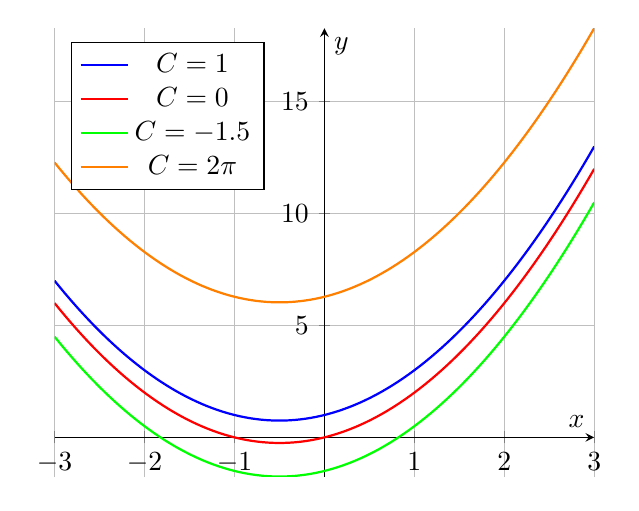
\begin{tikzpicture}
    \begin{axis}[
        xlabel={$x$},
        ylabel={$y$},
        axis lines=middle,
        grid=major,
        legend pos=north west,
        domain=-3:3,
        samples=100
    ]
    \addplot[blue, thick] {x^2 + x + 1};
    \addlegendentry{$C = 1$}
    
    \addplot[red, thick] {x^2 + x};
    \addlegendentry{$C = 0$}
    
    \addplot[green, thick] {x^2 + x - 1.5};
    \addlegendentry{$C = -1.5$}
    
    \addplot[orange, thick] {x^2 + x + 2*pi};
    \addlegendentry{$C = 2\pi$}
    \end{axis}
\end{tikzpicture}
\end{center}

To select a specific solution from the general solution, we need an initial condition: \( \boxed{y(t_I) = y_I} \).

The pair \( y' = f(t) \) with \( y(t_I) = y_I \) is called an Initial Value Problem (IVP).

\textbf{Example: Solve the IVP}

\[
\frac{dy}{dx} = 2x + 1 \quad \text{with} \quad y(0) = 2
\]

\textbf{Solution:}

Start with the general solution:

\[
y = x^2 + x + C
\]

Using the initial condition \( y(0) = 2 \):

\[
2 = 0^2 + 0 + C \quad \Rightarrow \quad C = 2
\]

Thus, the specific solution is:

\[
y = x^2 + x + 2
\]

\subsubsection*{Interval of Definition/Existence}

The interval of definition/existence of a solution to an IVP is the \textbf{largest} interval \( (a, b) \) where:

\begin{itemize}
    \item \( t_I \in (a, b) \)
    \item \( f(t) \) is continuous on \( (a, b) \)
\end{itemize}

\section*{Chapter 2: Linear Equations}

These look like:

\[
p(t) y' + q(t) y = r(t) \quad \text{where } p(t) \neq 0 \text{ for the values of } t \text{ we are considering.}
\]

In standard form:

\[
y' = -\frac{q(t)}{p(t)} y + \frac{r(t)}{p(t)}
\]

Let:

\[
a(t) = \frac{q(t)}{p(t)}, \quad f(t) = \frac{r(t)}{p(t)}
\]

We write it as:

\[
y' + a(t) y = f(t)
\]

Here, \( f(t) \) is called the forcing function.

If \( f(t) = 0 \), the ODE is called homogeneous; otherwise, it is non-homogeneous.

\subsection*{Recipe for Solving First-Order Linear ODEs}

Given:

\[
y' + a(t) y = f(t)
\]

1. Choose an antiderivative \( A(t) \) of \( a(t) \).
2. Multiply both sides by \( e^{A(t)} \):

\[
e^{A(t)} y' + a(t) e^{A(t)} y = f(t) e^{A(t)}
\]

Let:

\[
f(t) e^{A(t)} = g(t)
\]

This simplifies to:

\[
\frac{d}{dt} \left( e^{A(t)} y \right) = g(t)
\]

3. Integrate both sides:

\[
e^{A(t)} y = G(t) + C \quad \Rightarrow \quad y = e^{-A(t)} G(t) + C e^{-A(t)}
\]

This is the general solution.

\textbf{Example:} Solve the ODE

\[
\frac{dy}{dt} = -y
\]

1. Rewrite as \( y' + y = 0 \).
2. Here, \( a(t) = 1 \), so choose \( A(t) = t \).
3. Multiply both sides by \( e^t \):

\[
e^t y' + e^t y = 0 \quad \Rightarrow \quad \frac{d}{dt} (e^t y) = 0
\]

4. Integrate:

\[
e^t y = C \quad \Rightarrow \quad y = C e^{-t}
\]

This is the general solution.

\textbf{Example:} Consider the ODE

\[
y' = -y + e^t
\]

1. Rewrite as \( y' + y = e^t \).
2. Here, \( a(t) = 1 \), so choose \( A(t) = t \).
3. Multiply both sides by \( e^t \):

\[
e^t y' + e^t y = e^{2t} \quad \Rightarrow \quad \frac{d}{dt} (e^t y) = e^{2t}
\]

4. Integrate:

\[
e^t y = \frac{1}{2} e^{2t} + C \quad \Rightarrow \quad y = \frac{1}{2} e^t + C e^{-t}
\]

This is the general solution.

\textbf{Example: Solve the IVP}

\[
\frac{dx}{dt} + \cos(t)x = \cos(t) \quad \text{with} \quad x\left(\frac{\pi}{2}\right) = 0
\]

\textbf{Solution:}

1. Here, \( a(t) = \cos(t) \), so choose \( A(t) = \sin(t) \).
2. Multiply both sides by \( e^{\sin(t)} \):

\[
e^{\sin(t)} x' + \cos(t) e^{\sin(t)} x = \cos(t) e^{\sin(t)}
\]

This simplifies to:

\[
\frac{d}{dt} \left( e^{\sin(t)} x \right) = \cos(t) e^{\sin(t)}
\]

3. Integrate:

\[
e^{\sin(t)} x = \int \cos(t) e^{\sin(t)} \, dt = e^{\sin(t)} + C
\]

Thus,

\[
x = 1 + C e^{-\sin(t)}
\]

4. Apply the initial condition \( x\left(\frac{\pi}{2}\right) = 0 \):

\[
0 = 1 + C e^{-1} \quad \Rightarrow \quad C = -e
\]

Thus, the specific solution is:

\[
x = 1 - e^{1 - \sin(t)}
\]

\section*{Lecture 2, 8/29/2024}

I.2 (continued)

\section*{Problem Statement}

Consider the initial value problem (IVP):

\[
y' + a(t)y = f(t), \quad y(t_I) = y_I
\]

\textbf{Theorem:}  
If \( a(t) \) and \( f(t) \) are continuous over the interval \( (a, b) \) and \( t_I \in (a, b) \), then there is a unique solution to the IVP that is continuous on \( (a, b) \), and it's given by our method.

\section*{Example}

Consider the differential equation:

\[
z' + \cot(t)z = \frac{1}{\ln(t^2)}, \quad z(4) = 3
\]

Find the largest interval on which we can guarantee a unique continuous solution to this IVP.

\section*{Solution}

The function \( \ln(t^2) \) is continuous on \( (-\infty, 0) \) and \( (0, \infty) \), but \( \frac{1}{\ln(t^2)} \) is discontinuous at \( t = 0 \) and when \( \ln(t^2) = 0 \), i.e., \( t = \pm 1 \).

The function \( \cot(t) \) has discontinuities at multiples of \( \pi \).

The largest interval of continuity that includes \( t = 4 \) is \( (\pi, 2\pi) \).


\begin{center}
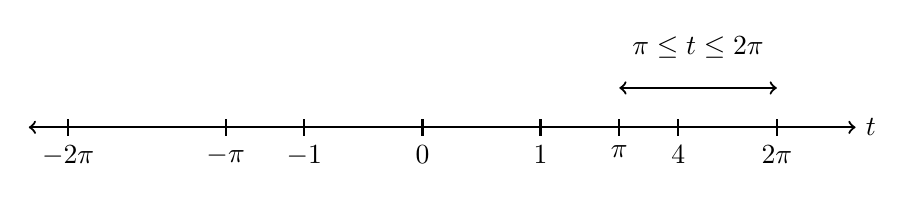
\begin{tikzpicture}

% Draw the line
\draw[thick, <->] (-5,0) -- (5.5,0) node[right] {$t$};

% Mark and label specific points
\foreach \x/\xtext in {-4.5/$-2\pi$, -2.5/$-\pi$, -1.5/$-1$, 0/$0$, 1.5/$1$, 2.5/$\pi$, 4.5/$2\pi$}
  \draw[thick] (\x,3pt) -- (\x,-3pt) node[below] {\xtext};

% Mark the point 4
\draw[thick] (3.25,3pt) -- (3.25,-3pt) node[below] {$4$};

% Draw the interval of continuity
\draw[thick,<->] (2.5,0.5) -- (4.5,0.5);
\node at (3.5,0.75) [above] {$\pi \leq t \leq 2\pi$};

\end{tikzpicture}
\end{center}


\section*{I.3: Separable Equation}

A first-order ordinary differential equation (ODE) is \textbf{separable} if it can be written in the form:

\[
y' = f(t)g(y)
\]

\textbf{Example:}

Consider the differential equation:

\[
y' = 2ty^2 + 3t^2y^2
\]

We can factor this as:

\[
y' = (2t + 3t^2)y^2
\]

Here, we have:

\[
f(t) = 2t + 3t^2, \quad g(y) = y^2
\]

An ODE of the form \( y' = g(y) \) is called \textbf{autonomous}.

A solution is called \textbf{stationary} if it is constant. If \( y = C \) is a stationary solution, then:

\[
y' = 0 \Rightarrow \boxed{0 = g(C)}
\]

\textbf{Example:}

Consider the equation:

\[
y' = 4y - y^3
\]

To find the stationary solutions, set:

\[
4y - y^3 = 0 \Rightarrow y(4 - y^2) = 0 \Rightarrow y(2 - y)(2 + y) = 0
\]

Thus, the stationary solutions are:

\[
y = 0, \quad y = 2, \quad y = -2
\]




\section*{Non-Stationary Solutions}

To find non-stationary solutions of the equation \( y' = g(y) \), we proceed as follows:

\[
y' = g(y) \quad \Rightarrow \quad \frac{1}{g(y)} y' = 1 
\]

Taking the integral on both sides:

\[
\int \frac{1}{g(y)} y' \, dt = \int 1 \, dt
\]

This simplifies to:

\[
\int \frac{1}{g(y)} \, dy = t + C
\]

The result is an implicit equation for our solution.

\textbf{Why can we divide by \( g(y) \)?}  
\( g(y) = 0 \) corresponds to stationary solutions, and we are looking for non-stationary solutions, i.e., \( g(y) \neq 0 \).

\section*{Example: Find All Solutions to \( y' = y^2 \)}

\textbf{Stationary Solutions:}  
Set \( y^2 = 0 \), which implies \( y = 0 \).

\textbf{Non-Stationary Solutions:}

Starting with the equation:

\[
\frac{1}{y^2} y' = 1
\]

Integrate both sides:

\[
\int \frac{1}{y^2} y' \, dt = \int 1 \, dt
\]

This simplifies to:

\[
\int \frac{1}{y^2} \, dy = t + C
\]

Evaluating the integral:

\[
-\frac{1}{y} = t + C
\]

We can find an explicit solution:

\[
-y = \frac{1}{t + C} \quad \Rightarrow \quad y = -\frac{1}{t + C}
\]



Each solution \( y = -\frac{1}{t + C} \) actually represents two solutions, one defined on \( (-\infty, -C) \) and the other on \( (-C, \infty) \).

\textbf{Note:} Our solution is discontinuous even though all functions in the original equation \( y' = y^2 \) are continuous.

\section*{General Separable Equations}

Consider the general separable equation:

\[
y' = f(t)g(y)
\]

If \( g(c) = 0 \), then \( y = c \) is a stationary solution (so set g(y) = 0).

For non-stationary solutions:

\[
\frac{1}{g(y)} y' = f(t)
\]

Taking the integral on both sides:

\[
\int \frac{1}{g(y)} y' \, dt = \int f(t) \, dt
\]

This simplifies to:

\[
\int \frac{1}{g(y)} \, dy = F(t) + C
\]

\section*{Example: Find All Solutions to \( \frac{dz}{dx} = \frac{3x + xz^2}{z + x^2z} \)}

First, rewrite the equation:

\[
\frac{dz}{dx} = \frac{x}{1 + x^2} \cdot \frac{3 + z^2}{z}
\]

Thus, we identify:

\[
f(x) = \frac{x}{1 + x^2}, \quad g(z) = \frac{3 + z^2}{z}
\]

\textbf{Stationary Solutions:}  
Set \( g(z) = 0 \):

\[
\frac{3 + z^2}{z} = 0 \quad \Rightarrow \quad 3 + z^2 = 0
\]

This equation has no real solution, so there are no stationary solutions.

\textbf{Non-Stationary Solutions:}

Start with:

\[
\frac{1}{g(z)} \frac{dz}{dx} = f(x)
\]

Which simplifies to:

\[
\frac{z}{3 + z^2} \cdot \frac{dz}{dx} = \frac{x}{1 + x^2}
\]

Integrate both sides:

\[
\int \frac{z}{3 + z^2} \frac{dz}{dx} \, dx = \int \frac{x}{1 + x^2} \, dx
\]

Use substitution:

- Let \( u = 3 + z^2 \), then \( du = 2z \, dz \).
- Let \( v = 1 + x^2 \), then \( dv = 2x \, dx \).

The integrals become:

\[
\int \frac{1}{2u} du = \int \frac{1}{2v} dv
\]

This integrates to:

\[
\frac{1}{2} \ln|u| = \frac{1}{2} \ln|v| + C
\]

Substituting back \( u \) and \( v \):

\[
\frac{1}{2} \ln|3 + z^2| = \frac{1}{2} \ln|1 + x^2| + C
\]



\section*{Initial Value Problems (IVPs)}

\textbf{Example:} Solve the initial value problem:

\[
y' = ty^2 - ty, \quad y(1) = 2
\]

We can factor the equation as:

\[
y' = t(y^2 - y)
\]

\textbf{Stationary Solutions:}  
Set \( y^2 - y = 0 \):

\[
y(y - 1) = 0 \quad \Rightarrow \quad y = 0 \quad \text{or} \quad y = 1
\]

Neither \( y = 0 \) nor \( y = 1 \) satisfies the initial condition \( y(1) = 2 \).

\begin{center}
\begin{tikzpicture}
    \draw[thick,->] (-1,0) -- (3,0) node[right] {$t$};
    \draw[thick,->] (0,-1) -- (0,3) node[above] {$y$};
    
    \draw[blue,thick] (-1,1) -- (3,1) node[below right] {$y=1$};
    \draw[red,thick] (-1,0) -- (3,0) node[below right] {$y=0$};

    \node at (1,2) [circle,fill,inner sep=1.5pt,label=above:{$(1,2)$}] {};
\end{tikzpicture}
\end{center}

As shown in the graph, neither \( y = 0 \) nor \( y = 1 \) passes through the point \( (1, 2) \).

\textbf{Other Solutions:}  
We solve the differential equation for non-stationary solutions:

\[
\frac{1}{y^2 - y} \frac{dy}{dt} = t \quad \Rightarrow \quad \frac{1}{y^2 - y} \, dy = t \, dt
\]

Integrate both sides:

\[
\int \frac{1}{y^2 - y} \, dy = \int t \, dt
\]

Using partial fractions:

\[
\frac{1}{y(y-1)} = \frac{A}{y} + \frac{B}{y-1}
\]

This leads to:

\[
1 = A(y - 1) + B(y) 
\]

By guessing \( A = -1 \) and \( B = 1 \), we get:

\[
\int \left( -\frac{1}{y} + \frac{1}{y-1} \right) dy = \int t \, dt
\]

Integrating both sides:

\[
-\ln|y| + \ln|y - 1| = \frac{t^2}{2} + C
\]

Using the logarithm property \( \ln(a) - \ln(b) = \ln\left(\frac{a}{b}\right) \), this simplifies to:

\[
\ln\left|\frac{y - 1}{y}\right| = \frac{t^2}{2} + C
\]

\textbf{Applying the Initial Condition:}  
Given \( y(1) = 2 \):

\[
\ln\left|\frac{2 - 1}{2}\right| = \frac{1^2}{2} + C
\]

\[
\ln\left(\frac{1}{2}\right) = \frac{1}{2} + C \quad \Rightarrow \quad C = \ln\left(\frac{1}{2}\right) - \frac{1}{2}
\]

Substituting \( C \) back into the equation:

\[
\ln\left|\frac{y - 1}{y}\right| = \frac{t^2}{2} + \ln\left(\frac{1}{2}\right) - \frac{1}{2}
\]




\section*{Uniqueness and Existence Theorem}

If \( f(t) \) is continuous on \( (a, b) \) and \( g(y) \) is continuous and differentiable on \( (c, d) \), then for every \( t_I \in (a, b) \) and \( y_I \in (c, d) \), there exists a unique continuous solution to the equation

\[
y' = f(t)g(y)
\]

with the initial condition \( y(t_I) = y_I \), defined on some interval around \( t_I \). The solution is determined by our method.

\section*{Example}

Consider the differential equation:

\[
\frac{dy}{dt} = 3y^{2/3}, \quad y(0) = 0
\]

\textbf{Stationary Solution:}  
\( y = 0 \) is a stationary solution, and it solves our initial value problem (IVP).

However, \( g(y) = 3y^{2/3} \) is not differentiable at \( y = 0 \), so we might have other solutions.

\textbf{Finding Other Solutions:}

\[
\frac{1}{3y^{2/3}} \frac{dy}{dt} = 1
\]

Integrating both sides:

\[
\int \frac{1}{3y^{2/3}} \, dy = \int 1 \, dt
\]

This simplifies to:

\[
y^{1/3} = t + C
\]

Raising both sides to the power of 3:

\[
y = (t + C)^3
\]

\textbf{Applying the Initial Condition:}  
For \( y(0) = 0 \), we get \( C = 0 \), so:

\[
y = t^3
\]

Thus, \( y = t^3 \) also solves our IVP.


\section*{Lecture 3, Tuesday 9/3/2024}


\textbf{Quiz tomorrow:} Up to Section I.3

\section*{I.4. Theory}

Consider Initial Value Problems (IVPs) of the form:
\[
y' = f(t,y), \quad y(t_i) = y_i
\]

We say the problem is \textit{well-posed} if:

\begin{enumerate}
    \item There exists a solution
    \item The solution is unique
    \item The solution depends continuously on the initial conditions
\end{enumerate}

\subsection*{Existence and Uniqueness}

Consider a set $S$ of points in the $(t,y)$ plane.

\begin{figure}[h]
    \centering
    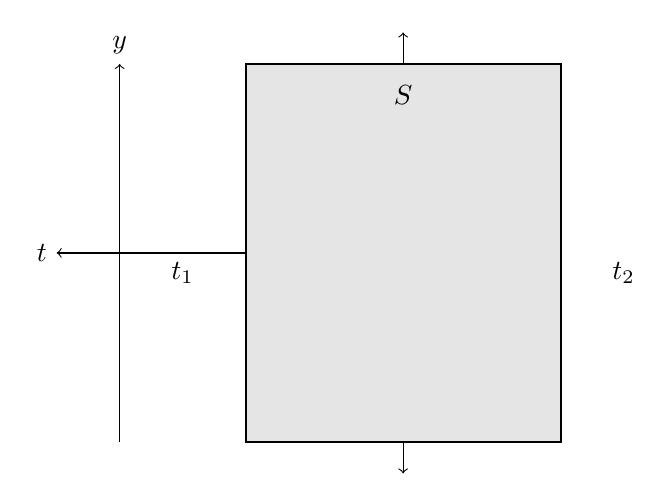
\begin{tikzpicture}[scale=0.8]
        % Draw the axes
        \draw[->] (6,0) -- (-1,0) node[left] {$t$};
        \draw[->] (0,-3) -- (0,3) node[above] {$y$};
        
        % Draw the vertical rectangle S
        \fill[gray!20] (2,-3) rectangle (7,3);
        \draw[thick] (2,-3) rectangle (7,3);
        
        % Label the set S
        \node at (4.5,2.5) {$S$};
        
        % Label the t-coordinates
        \node[below] at (1,0) {$t_1$};
        \node[below] at (8,0) {$t_2$};
        
        % Add arrows to indicate infinite extension in y-direction
        \draw[->] (4.5,3) -- (4.5,3.5);
        \draw[->] (4.5,-3) -- (4.5,-3.5);
    \end{tikzpicture}
    \caption{The set $S$ in the $(t,y)$ plane}
    \label{fig:set_S}
\end{figure}

If $f(t,y)$ is continuous on $S$ and $\frac{\partial f}{\partial y}$ is continuous on $S$, then for any $(t_i, y_i) \in S$, there exists a unique continuous solution $Y(t)$ to the initial value problem:
\[
\begin{cases}
y' = f(t,y) \\
Y(t_i) = y_i
\end{cases}
\]
defined over some interval $(a,b)$ containing $t_i$.

Moreover, the interval $(a,b)$ can be extended as long as $(t, Y(t))$ remains inside $S$.

\textbf{Example:} Consider $y' = \frac{\sin(t+ty^2)}{1+t^2}$, $y(0) = 1$

Let's show that there is a unique solution defined on $(-1, 1)$.

\textbf{Solution:} 
For $f(t, y) = \frac{\sin(t+ty^2)}{1+t^2}$, $f$ is continuous except at $t = \pm 1$.

$\frac{\partial f}{\partial y} = \frac{2ty\cos(t+ty^2)}{1+t^2}$, which is also continuous except at $t = \pm 1$.

By the Existence and Uniqueness Theorem, since $f$ and $\frac{\partial f}{\partial y}$ are continuous on $S$, there exists a unique solution $y(t)$ to the initial value problem, defined on some interval containing $t=0$. This interval can be extended as long as $(t,y(t))$ remains inside $S$, which in this case is the entire interval $(-1,1)$.

Since $t_i = 0$, $y_i = 1 \implies (0,1) \in S$, the theorem tells us we have a unique solution $Y(t)$ defined on a larger $(a, b)$ such that $y(t)$ remains inside $S$.

Since any solution will not leave $S$ as long as $-1 < t < 1$, we get $(a,b) = (-1, 1)$.

So, we choose $S$ as follows:

\begin{figure}[h]
    \centering
    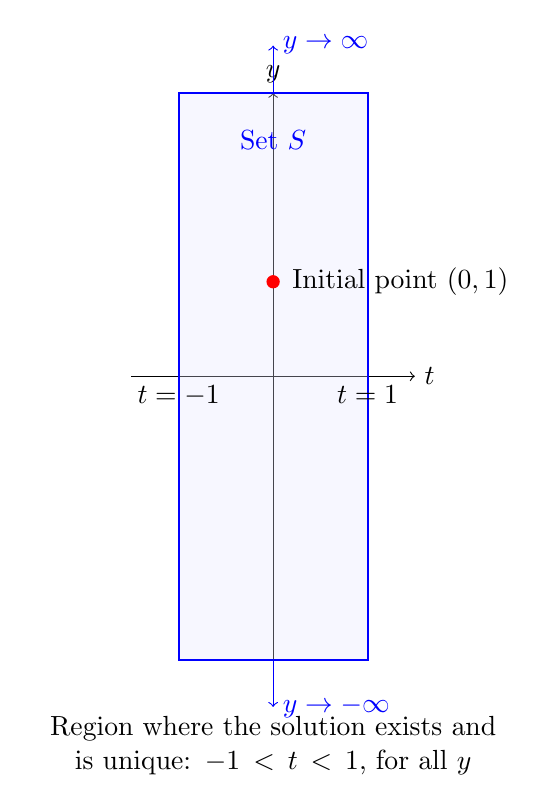
\begin{tikzpicture}[scale=1.2]
        % Draw the axes
        \draw[->] (-1.5,0) -- (1.5,0) node[right] {$t$};
        \draw[->] (0,-3) -- (0,3) node[above] {$y$};
        
        % Draw the vertical rectangle S with transparent fill
        \fill[blue!10, opacity=0.3] (-1,-3) rectangle (1,3);
        \draw[thick, blue] (-1,-3) rectangle (1,3);
        
        % Label the set S
        \node[blue] at (0,2.5) {Set $S$};
        
        % Label the t-coordinates
        \node[below] at (-1,0) {$t=-1$};
        \node[below] at (1,0) {$t=1$};
        
        % Add arrows and labels to indicate infinite extension in y-direction
        \draw[->, blue] (0,3) -- (0,3.5) node[right] {$y \to \infty$};
        \draw[->, blue] (0,-3) -- (0,-3.5) node[right] {$y \to -\infty$};
        
        % Mark the initial point (0,1)
        \fill[red] (0,1) circle (2pt);
        \node[right] at (0.1,1) {Initial point $(0,1)$};
        
        % Add explanation
        \node[text width=6cm, align=center, below] at (0,-3.5) 
        {Region where the solution exists and is unique: $-1 < t < 1$, for all $y$};
    \end{tikzpicture}
    \caption{Set $S$ where the solution to the differential equation is guaranteed to exist and be unique}
    \label{fig:set_S_example}
\end{figure}

\pagebreak

\textbf{Example:} Consider the differential equation $y' = \frac{1}{t^2 + y^2 - 1}$, with initial condition $y(0) = 0$. Find the set $S$ where the solution is guaranteed to exist and be unique.

\textbf{Solution:} 
The function $f(t,y) = \frac{1}{t^2 + y^2 - 1}$ is discontinuous when $t^2 + y^2 = 1$. This equation describes a circle with radius 1 centered at the origin.

The set $S$ where the solution exists and is unique should be the interior of this circle, excluding the circle itself. We can represent this as:

\[S = \{(t,y) : t^2 + y^2 < 1\}\]

Let's visualize this set:

\begin{figure}[h]
    \centering
    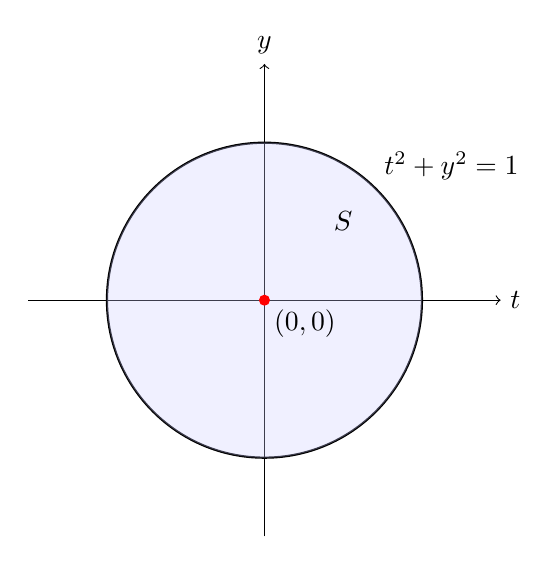
\begin{tikzpicture}[scale=2]
        % Draw the axes
        \draw[->] (-1.5,0) -- (1.5,0) node[right] {$t$};
        \draw[->] (0,-1.5) -- (0,1.5) node[above] {$y$};
        
        % Draw the circle t^2 + y^2 = 1
        \draw[thick] (0,0) circle (1);
        
        % Fill the interior of the circle (set S) with transparent highlight
        \fill[blue!20, opacity=0.3] (0,0) circle (1);
        
        % Label the set S
        \node at (0.5,0.5) {$S$};
        
        % Mark the initial point (0,0)
        \fill[red] (0,0) circle (1pt);
        \node[below right] at (0,0) {$(0,0)$};
        
        % Label the circle
        \node[above right] at (0.7,0.7) {$t^2 + y^2 = 1$};
    \end{tikzpicture}
    \caption{Set $S$ for the given differential equation}
    \label{fig:set_S_circle_example}
\end{figure}

The solution is guaranteed to exist and be unique within this circular region $S$, but not on or outside the boundary where $t^2 + y^2 = 1$.

\textbf{Example:} Consider the differential equation $y' = \frac{1}{t^2 + y^2 - 1}$, with initial condition $y(0) = 3$. Let's visualize the set $S$ where the solution is guaranteed to exist and be unique.

\textbf{Solution:} 
The function $f(t,y) = \frac{1}{t^2 + y^2 - 1}$ is discontinuous when $t^2 + y^2 = 1$. This equation describes a circle with radius 1 centered at the origin.

The set $S$ where the solution exists and is unique should be the region outside this circle, including the initial point $(0,3)$. We can represent this as:

\[S = \{(t,y) : t^2 + y^2 > 1\}\]

Let's visualize this set:

\pagebreak
\begin{figure}[h]
    \centering
    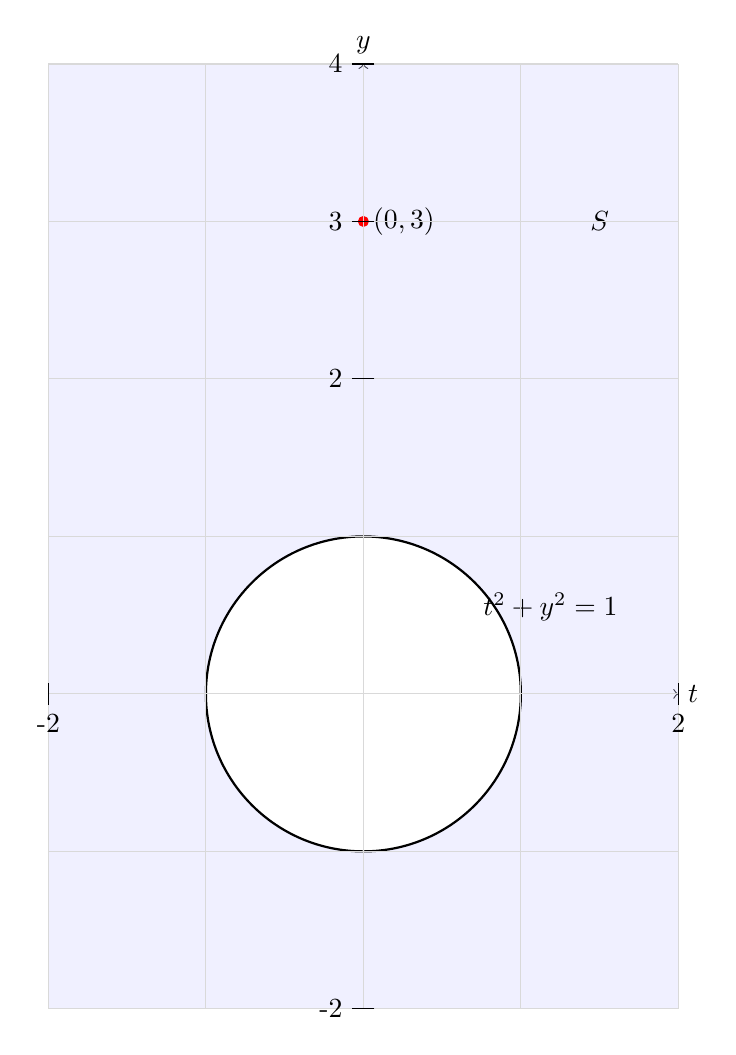
\begin{tikzpicture}[scale=2]
        % Draw the axes
        \draw[->] (-2,0) -- (2,0) node[right] {$t$};
        \draw[->] (0,-2) -- (0,4) node[above] {$y$};
        
        % Fill the exterior of the circle (set S) with transparent highlight
        \begin{scope}
            \clip (-2,-2) rectangle (2,4);
            \fill[blue!20, opacity=0.3] (-2,-2) rectangle (2,4);
            \fill[white] (0,0) circle (1);
        \end{scope}
        
        % Draw the circle t^2 + y^2 = 1
        \draw[thick] (0,0) circle (1);
        \node[anchor=north west] at (0.7,0.7) {$t^2 + y^2 = 1$};
        
        % Label the set S
        \node at (1.5,3) {$S$};
        
        % Mark the initial point (0,3)
        \fill[red] (0,3) circle (1pt);
        \node[right] at (0,3) {$(0,3)$};
        
        % Add grid lines for better visualization
        \draw[gray!30, step=1] (-2,-2) grid (2,4);
        
        % Label the axes
        \foreach \x in {-2,2}
            \draw (\x,2pt) -- (\x,-2pt) node[below] {\x};
        \foreach \y in {-2,2,3,4}
            \draw (2pt,\y) -- (-2pt,\y) node[left] {\y};
    \end{tikzpicture}
    \caption{Set $S$ for the given differential equation with $y(0) = 3$}
    \label{fig:set_S_circle_example_y0_3}
\end{figure}

The solution is guaranteed to exist and be unique within the region $S$, which is the area outside the circle $t^2 + y^2 = 1$, including the initial point $(0,3)$.


\pagebreak

\section{I.5 - Graphical Methods}

\subsection{Phase Portraits for Autonomous Equations}

Consider the autonomous differential equation:

\[
\frac{dy}{dt} = g(y)
\]

Our goal is to describe the qualitative behavior of solutions without explicitly solving the equation.

\begin{itemize}
    \item When $g(y) = 0$:
        \begin{itemize}
            \item $y' = 0$
            \item We have a stationary solution
        \end{itemize}
    
    \item When $g(y) > 0$:
        \begin{itemize}
            \item $y' > 0$
            \item The solution is increasing
        \end{itemize}
    
    \item When $g(y) < 0$:
        \begin{itemize}
            \item $y' < 0$
            \item The solution is decreasing
        \end{itemize}
\end{itemize}


\subsection*{Example: $y' = 4y - y^3$}

Let's analyze the differential equation $y' = 4y - y^3$.

\begin{enumerate}
    \item First, we find the stationary solutions:
    \[
    4y - y^3 = y(4 - y^2) = y(2-y)(2+y) = 0
    \]
    Thus, the stationary solutions are $y = 0, \pm 2$.

    \item Next, we determine the sign of $g(y) = 4y - y^3$ between these zeros:
    \begin{align*}
        g(1) &= 4(1) - (1)^3 = 3 > 0 \\
        g(3) &= 4(3) - (3)^3 = 12 - 27 = -15 < 0 \\
        g(-3) &= 4(-3) - (-3)^3 = -12 + 27 = 15 > 0 \\
        g(-1) &= 4(-1) - (-1)^3 = -4 + 1 = -3 < 0
    \end{align*}
\end{enumerate}

Based on this analysis, we can create a phase portrait:

\begin{figure}[h]
    \centering
    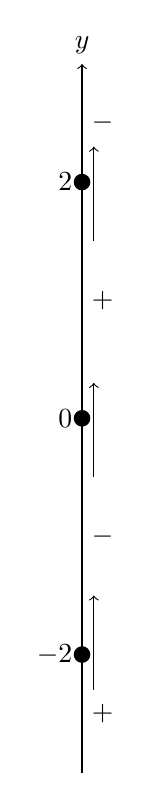
\begin{tikzpicture}[scale=1.5]
        % Draw y-axis
        \draw[->] (0,-3) -- (0,3) node[above] {$y$};
        
        % Plot points and labels
        \foreach \y/\label in {2/2, 0/0, -2/-2} {
            \fill (0,\y) circle (2pt);
            \node[left] at (0,\y) {$\y$};
        }
        
        % Add + and - signs
        \node[right] at (0,2.5) {$-$};
        \node[right] at (0,1) {$+$};
        \node[right] at (0,-1) {$-$};
        \node[right] at (0,-2.5) {$+$};
        
        % Add arrows to show direction
        \draw[->] (0.1,1.5) -- (0.1,2.3);
        \draw[->] (0.1,-0.5) -- (0.1,0.3);
        \draw[->] (0.1,-2.3) -- (0.1,-1.5);
    \end{tikzpicture}
    \caption{Phase portrait for $y' = 4y - y^3$}
    \label{fig:phase_portrait_4y_minus_y3}
\end{figure}

The phase portrait shows:
\begin{itemize}
    \item Solutions increase when $y \in (-\infty, -2) \cup (0, 2)$
    \item Solutions decrease when $y \in (-2, 0) \cup (2, \infty)$
    \item Stationary solutions at $y = 0, \pm 2$
\end{itemize}




This diagram is called a phase portrait or phase line. It provides valuable information about the behavior of solutions $y(t)$ for different initial conditions:

\begin{itemize}
    \item For $y(t)$ starting in $(-\infty, -2)$:
        \begin{itemize}
            \item $y(t)$ increases as $t$ increases
            \item $y(t) \rightarrow -2$ as $t \rightarrow \infty$ (asymptotically approaching -2)
        \end{itemize}
    
    \item For $y(t)$ starting in $(-2, 0)$:
        \begin{itemize}
            \item $y(t)$ is decreasing
            \item $y(t) \rightarrow -2$ as $t \rightarrow \infty$
        \end{itemize}
    
    \item For $y(t)$ starting in $(0, 2)$:
        \begin{itemize}
            \item $y(t)$ is increasing
            \item $y(t) \rightarrow 2$ as $t \rightarrow \infty$ (asymptotically approaching 2)
        \end{itemize}
    
    \item For $y(t)$ starting in $(2, \infty)$:
        \begin{itemize}
            \item $y(t)$ is decreasing
            \item $y(t) \rightarrow 2$ as $t \rightarrow \infty$ (asymptotically approaching 2)
        \end{itemize}
\end{itemize}


Sketch solutions:

\begin{figure}[h]
    \centering
    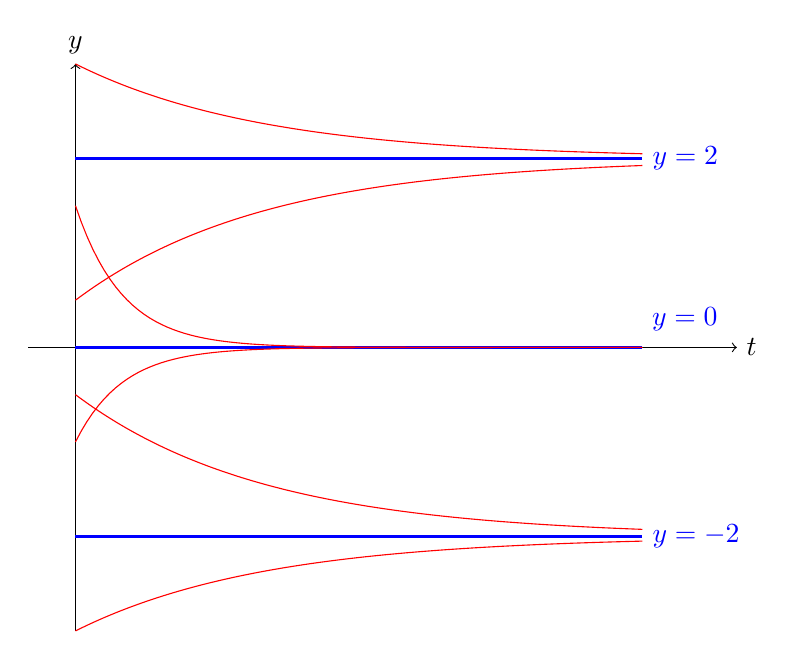
\begin{tikzpicture}[scale=1.2]
        % Axes
        \draw[->] (-0.5,0) -- (7,0) node[right] {$t$};
        \draw[->] (0,-3) -- (0,3) node[above] {$y$};
        
        % Constant solutions
        \draw[thick, blue] (0,2) -- (6,2) node[right] {$y=2$};
        \draw[thick, blue] (0,0) -- (6,0) node[right] {};
        \draw[thick, blue] (0,-2) -- (6,-2) node[right] {$y=-2$};

        % Label for y=0
        \node[right, blue] at (6,0.3) {$y=0$};
        
        % Solutions approaching -2
        \draw[red] plot[domain=0:6, samples=100] (\x, {-2+1.5*exp(-\x/2)});
        \draw[red] plot[domain=0:6, samples=100] (\x, {-2-exp(-\x/2)});
        
        % Solutions approaching 2
        \draw[red] plot[domain=0:6, samples=100] (\x, {2-1.5*exp(-\x/2)});
        \draw[red] plot[domain=0:6, samples=100] (\x, {2+exp(-\x/2)});
        
        % Solution approaching 0
        \draw[red] plot[domain=0:6, samples=100] (\x, {1.5*exp(-2*\x)});
        \draw[red] plot[domain=0:6, samples=100] (\x, {-exp(-2*\x)});
    \end{tikzpicture}
    \caption{Sketch of solutions for $y' = 4y - y^3$}
    \label{fig:solutions_4y_minus_y3}
\end{figure}

This figure illustrates:
\begin{itemize}
    \item Constant solutions at $y=2$, $y=0$, and $y=-2$ (blue lines)
    \item Solutions approaching $y=2$ from above and below
    \item Solutions approaching $y=-2$ from above and below
    \item Solutions approaching $y=0$ from above and below
\end{itemize}

The red curves represent various solutions to the differential equation, showing how they behave over time depending on their initial conditions.

We classify stationary solutions as follows:

\begin{itemize}
    \item \textbf{Stable or attracting:} All nearby solutions move towards it as $t \rightarrow \infty$. 
          \\ (In this case: $y = \pm 2$)
    
    \item \textbf{Unstable or repelling:} All nearby solutions move away from it as $t \rightarrow \infty$. 
          \\ (In this case: $y = 0$)
    
    \item \textbf{Semi-stable:} Some solutions move towards it and some move away from it as $t \rightarrow \infty$.
\end{itemize}

\begin{figure}[h]
    \centering
    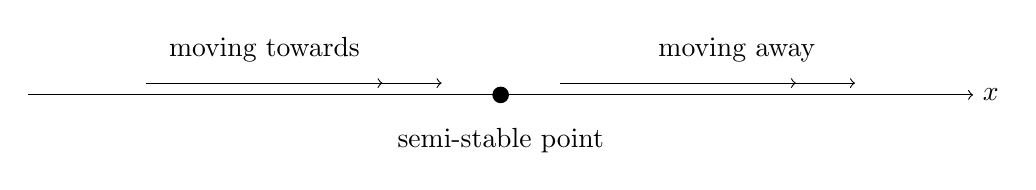
\begin{tikzpicture}[scale=1.5]
        % Draw the x-axis
        \draw[->] (-4,0) -- (4,0) node[right] {$x$};
        
        % Draw the semi-stable point
        \fill[black] (0,0) circle (2pt);
        \node[below] at (0,-0.2) {semi-stable point};
        
        % Draw arrows moving towards the point
        \draw[->] (-3,0.1) -- (-1,0.1);
        \draw[->] (-2.5,0.1) -- (-0.5,0.1);
        
        % Draw arrows moving away from the point
        \draw[->] (1,0.1) -- (3,0.1);
        \draw[->] (0.5,0.1) -- (2.5,0.1);
        
        % Labels
        \node[above] at (-2,0.2) {moving towards};
        \node[above] at (2,0.2) {moving away};
    \end{tikzpicture}
    \caption{Behavior near a semi-stable point}
    \label{fig:semi_stable_point}
\end{figure}



\textbf{Example:} Consider the differential equation $y' = y^2$

\begin{itemize}
    \item Stationary solution: $y = 0$
    \item For $y \neq 0$: $y^2 > 0$, implying solutions move away from $y = 0$
\end{itemize}

This example demonstrates an unstable stationary solution at $y = 0$.

\begin{figure}[h]
    \centering
    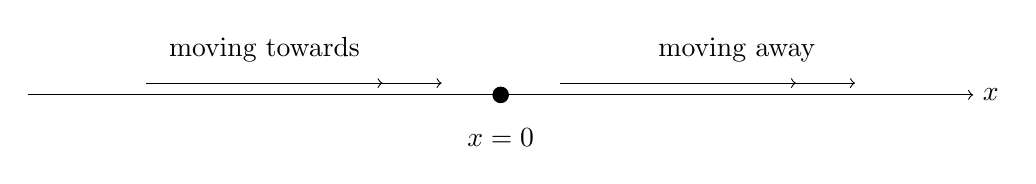
\begin{tikzpicture}[scale=1.5]
        % Draw the x-axis
        \draw[->] (-4,0) -- (4,0) node[right] {$x$};
        
        % Draw arrows moving towards the origin
        \draw[->] (-3,0.1) -- (-1,0.1);
        \draw[->] (-2.5,0.1) -- (-0.5,0.1);
        
        % Draw arrows moving away from the origin
        \draw[->] (1,0.1) -- (3,0.1);
        \draw[->] (0.5,0.1) -- (2.5,0.1);
        
        % Labels
        \node[above] at (-2,0.2) {moving towards};
        \node[above] at (2,0.2) {moving away};
        
        % Origin point
        \fill[black] (0,0) circle (2pt);
        \node[below] at (0,-0.2) {$x=0$};
    \end{tikzpicture}
    \caption{Behavior on x-axis for $y'=y^2$}
    \label{fig:x_axis_behavior}
\end{figure}

\begin{figure}[h]
    \centering
    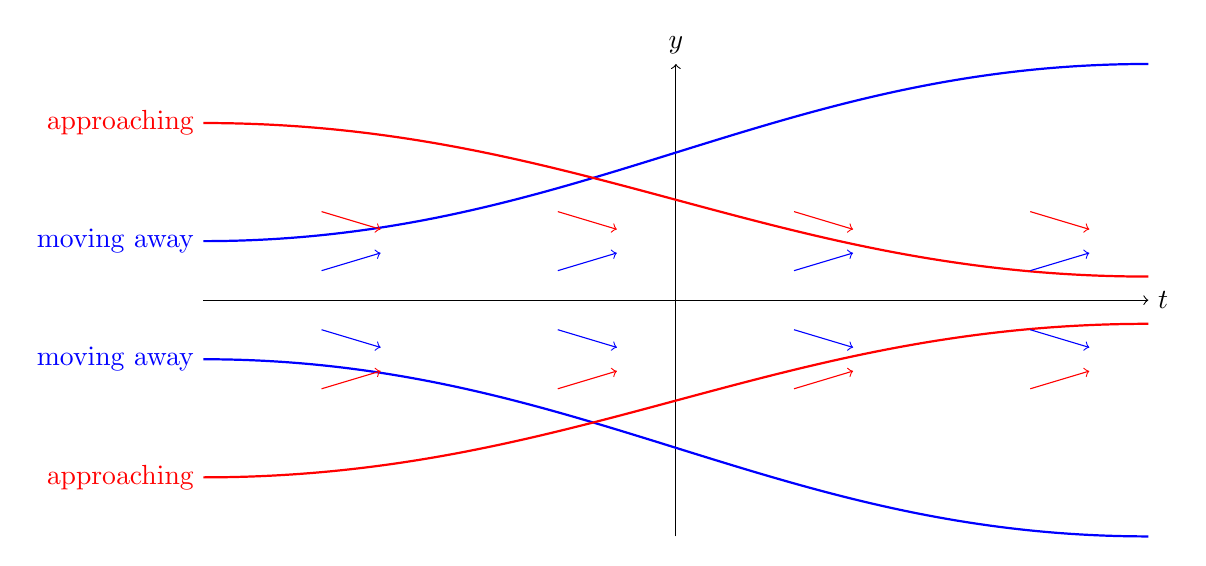
\begin{tikzpicture}[scale=1.5]
        % Draw the axes
        \draw[->] (-4,0) -- (4,0) node[right] {$t$};
        \draw[->] (0,-2) -- (0,2) node[above] {$y$};
        
        % Draw the y=0 line
        \draw[dashed] (-4,0) -- (4,0);
        
        % Draw solutions moving away from y=0
        \draw[blue, thick] (-4,0.5) to[out=0,in=180] (4,2);
        \draw[blue, thick] (-4,-0.5) to[out=0,in=180] (4,-2);
        
        % Draw solutions approaching y=0
        \draw[red, thick] (-4,1.5) to[out=0,in=180] (4,0.2);
        \draw[red, thick] (-4,-1.5) to[out=0,in=180] (4,-0.2);
        
        % Labels
        \node[blue, left] at (-4,0.5) {moving away};
        \node[blue, left] at (-4,-0.5) {moving away};
        \node[red, left] at (-4,1.5) {approaching};
        \node[red, left] at (-4,-1.5) {approaching};
        
        % Arrows indicating direction
        \foreach \x in {-3,-1,1,3} {
            \draw[->, blue] (\x,0.25) -- (\x+0.5,0.4);
            \draw[->, blue] (\x,-0.25) -- (\x+0.5,-0.4);
            \draw[->, red] (\x,0.75) -- (\x+0.5,0.6);
            \draw[->, red] (\x,-0.75) -- (\x+0.5,-0.6);
        }
    \end{tikzpicture}
    \caption{Behavior of solutions in t-y plane for $y'=y^2$}
    \label{fig:ty_plane_behavior}
\end{figure}

This figure illustrates the behavior of solutions to $y'=y^2$ near the stationary solution $y=0$. The blue curves represent solutions moving away from $y=0$, while the red curves represent solutions approaching $y=0$. This demonstrates that $y=0$ is an unstable or repelling stationary solution.



For stability think of a pendulum


\begin{figure}[h]
    \centering
    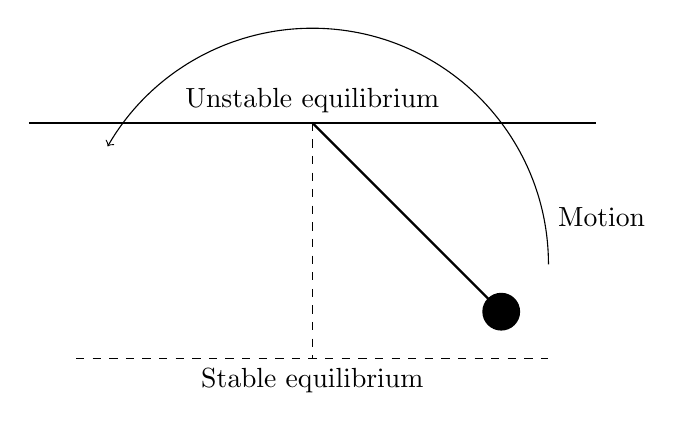
\begin{tikzpicture}[scale=1.2]
        % Draw the support
        \draw[thick] (-3,3) -- (3,3);
        
        % Draw the pendulum rod
        \draw[thick] (0,3) -- (2,1);
        
        % Draw the pendulum bob
        \fill[black] (2,1) circle (0.2);
        
        % Draw the arc to show motion
        \draw[->] (2.5,1.5) arc (0:150:2.5);
        
        % Label the stationary points
        \node[above] at (0,3) {Unstable equilibrium};
        \node[below] at (0,0.5) {Stable equilibrium};
        
        % Draw dashed lines to show equilibrium positions
        \draw[dashed] (0,3) -- (0,0.5);
        \draw[dashed] (-2.5,0.5) -- (2.5,0.5);
        
        % Label the motion
        \node[right] at (2.5,2) {Motion};
        
    \end{tikzpicture}
    \caption{Pendulum illustrating stable and unstable equilibrium points}
    \label{fig:pendulum}
\end{figure}

This figure illustrates a pendulum moving from right to left. The top position (vertically upright) represents an unstable equilibrium, while the bottom position represents a stable equilibrium. These correspond to the stationary solutions of the pendulum's differential equation.


unstable solution is pendulum at the top and stable is pendulum at the bottom





\subsection*{Example: Phase Line Analysis}

Consider the differential equation:

\[
y' = \frac{(y^2-1)(y-3)^2}{(y+3)^2}
\]

\textbf{Stationary Solutions:}
\begin{itemize}
    \item $y = -1$
    \item $y = 1$
    \item $y = 3$
\end{itemize}

\textbf{Note:} $y = -3$ is undefined in the equation.

We will now draw the phase line for this differential equation to analyze its behavior.

\begin{figure}[h]
    \centering
    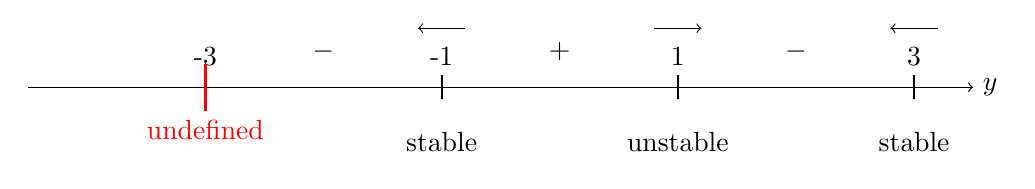
\begin{tikzpicture}[scale=1.5]
        % Draw the y-axis
        \draw[->] (-0.5,0) -- (7.5,0) node[right] {$y$};
        
        % Mark and label the points
        \foreach \x/\xtext in {1/-3, 3/-1, 5/1, 7/3}
            \draw[thick] (\x,-0.1) -- (\x,0.1) node[above] {\xtext};
        
        % Show the undefined point at y = -3
        \draw[red, thick] (1,-0.2) -- (1,0.2);
        \node[below, red] at (1,-0.2) {undefined};
        
        % Add + and - signs between points
        \node at (2,0.3) {$-$};
        \node at (4,0.3) {$+$};
        \node at (6,0.3) {$-$};
        
        % Add arrows to show stability
        \draw[->] (3.2,0.5) -- (2.8,0.5);
        \draw[->] (4.8,0.5) -- (5.2,0.5);
        \draw[<-] (6.8,0.5) -- (7.2,0.5);
        
        % Label stationary solutions
        \node[below] at (3,-0.3) {stable};
        \node[below] at (5,-0.3) {unstable};
        \node[below] at (7,-0.3) {stable};
    \end{tikzpicture}
    \caption{Phase line for $y' = (y^2-1)(y-3)^2 / (y+3)^2$}
    \label{fig:phase_line}
\end{figure}




Note: stability only applies to stationary solutions, not to undefined points.

Sketch
\begin{figure}[h]
    \centering
    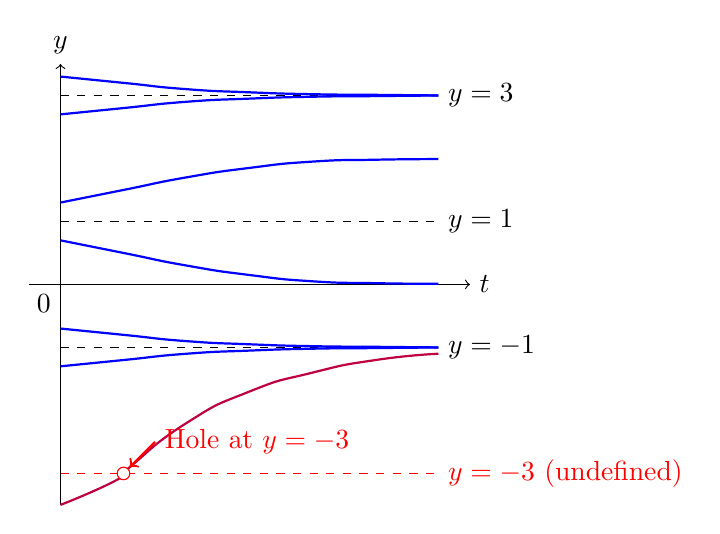
\begin{tikzpicture}[scale=0.8]
        % Draw the axes
        \draw[->] (-0.5,0) -- (6.5,0) node[right] {$t$};
        \draw[->] (0,-3.5) -- (0,3.5) node[above] {$y$};
        
        % Draw the horizontal lines for y = 3, 1, -1, -3
        \draw[dashed] (0,3) -- (6,3) node[right] {$y=3$};
        \draw[dashed] (0,1) -- (6,1) node[right] {$y=1$};
        \draw[dashed] (0,-1) -- (6,-1) node[right] {$y=-1$};
        \draw[dashed, red] (0,-3) -- (6,-3) node[right, red] {$y=-3$ (undefined)};
        
        % Draw some solution curves
        \draw[thick, blue] plot [smooth, tension=1] coordinates {(0,3.3) (1,3.2) (2,3.1) (3,3.05) (4,3.02) (5,3.01) (6,3)};
        \draw[thick, blue] plot [smooth, tension=1] coordinates {(0,2.7) (1,2.8) (2,2.9) (3,2.95) (4,2.98) (5,2.99) (6,3)};
        \draw[thick, blue] plot [smooth, tension=1] coordinates {(0,1.3) (1,1.5) (2,1.7) (3,1.85) (4,1.95) (5,1.98) (6,1.99)};
        \draw[thick, blue] plot [smooth, tension=1] coordinates {(0,0.7) (1,0.5) (2,0.3) (3,0.15) (4,0.05) (5,0.02) (6,0.01)};
        \draw[thick, blue] plot [smooth, tension=1] coordinates {(0,-0.7) (1,-0.8) (2,-0.9) (3,-0.95) (4,-0.98) (5,-0.99) (6,-1)};
        \draw[thick, blue] plot [smooth, tension=1] coordinates {(0,-1.3) (1,-1.2) (2,-1.1) (3,-1.05) (4,-1.02) (5,-1.01) (6,-1)};
        
        % Draw a line crossing y = -3 and approaching y = -1
        \draw[thick, purple] plot [smooth, tension=1] coordinates {(0,-3.5) (0.9,-3.1) (1.1,-2.9) (2,-2.2) (3,-1.7) (4,-1.4) (5,-1.2) (6,-1.1)};
       
        % Add a clear hole at y = -3
        \fill[white] (1,-3) circle (0.1);
        \draw[red] (1,-3) circle (0.1);
        
        % Add an arrow pointing to the hole
        \draw[->, red, thick] (1.5,-2.5) -- (1.1,-2.9);
        \node[red, right] at (1.5,-2.5) {Hole at $y=-3$};
        
        % Label the axes
        \node[below left] at (0,0) {0};
        
    \end{tikzpicture}
    \caption{Sketch of solutions for $y' = (y^2-1)(y-3)^2 / (y+3)^2$, including a solution crossing $y=-3$ with a clear hole}
    \label{fig:solution_sketch}
\end{figure}




\textbf{Example:} Consider the differential equation $y' = t - y^2$

\textbf{Procedure:} To sketch the slope field:
\begin{enumerate}
    \item Choose a representative selection of $(t, y)$ points.
    \item At each point $(t,y)$, draw an arrow with slope $t - y^2$.
    \item Connect the arrows to visualize solution curves.
\end{enumerate}

\textbf{Sample calculations:}
\begin{align*}
    \text{At } (0,0):& \quad t - y^2 = 0 \\
    \text{At } (1,0):& \quad t - y^2 = 1 \\
    \text{At } (-1,0):& \quad t - y^2 = -1 \\
    \text{At } (0,\pm 1):& \quad t - y^2 = -1
\end{align*}

Continue this process for other points to build a comprehensive slope field.

\begin{figure}[h]
    \centering
    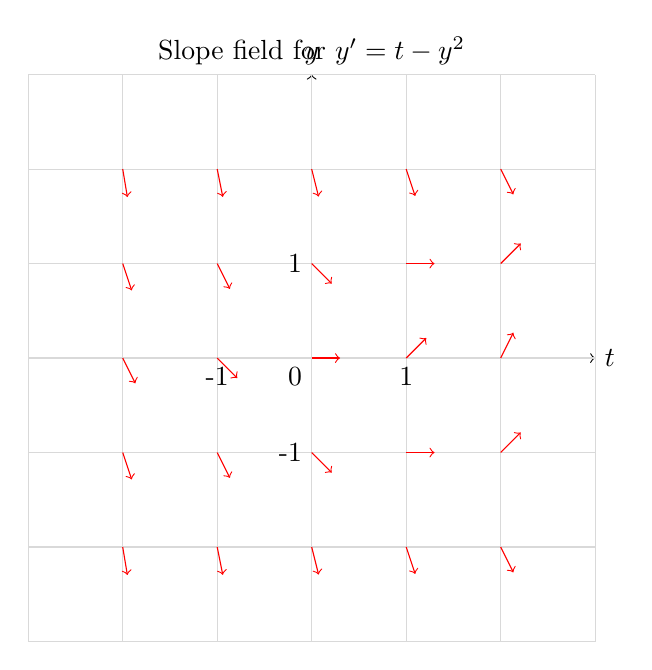
\begin{tikzpicture}[scale=1.2]
        % Draw the axes
        \draw[->] (-3,0) -- (3,0) node[right] {$t$};
        \draw[->] (0,-3) -- (0,3) node[above] {$y$};
        
        % Draw grid lines
        \draw[gray!30] (-3,-3) grid (3,3);
        
        % Draw arrows representing the slope field
        \foreach \x in {-2,-1,0,1,2} {
            \foreach \y in {-2,-1,0,1,2} {
                \pgfmathsetmacro{\slope}{\x - \y*\y}
                \draw[red,->] (\x,\y) -- ++({0.3*cos(atan(\slope))},{0.3*sin(atan(\slope))});
            }
        }
        
        % Label the axes
        \node[below left] at (0,0) {0};
        \node[below] at (1,0) {1};
        \node[below] at (-1,0) {-1};
        \node[left] at (0,1) {1};
        \node[left] at (0,-1) {-1};
        
        % Add title
        \node[above] at (0,3) {Slope field for $y' = t - y^2$};
    \end{tikzpicture}
    \caption{Slope field for the differential equation $y' = t - y^2$}
    \label{fig:slope_field}
\end{figure}


\begin{figure}[h]
    \centering
    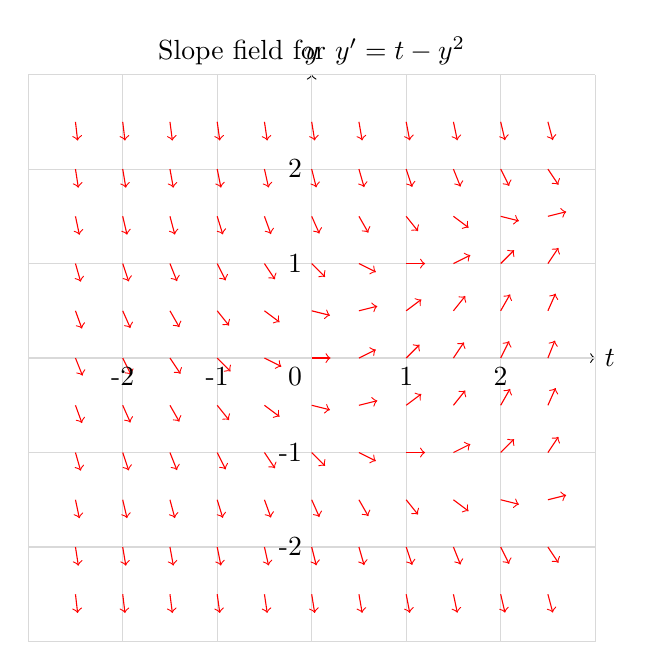
\begin{tikzpicture}[scale=1.2]
        % Draw the axes
        \draw[->] (-3,0) -- (3,0) node[right] {$t$};
        \draw[->] (0,-3) -- (0,3) node[above] {$y$};
        
        % Draw grid lines
        \draw[gray!30] (-3,-3) grid (3,3);
        
        % Draw arrows representing the slope field
        \foreach \x in {-2.5,-2,...,2.5} {
            \foreach \y in {-2.5,-2,...,2.5} {
                \pgfmathsetmacro{\slope}{\x - \y*\y}
                \draw[red,->] (\x,\y) -- ++({0.2*cos(atan(\slope))},{0.2*sin(atan(\slope))});
            }
        }
        
        % Label the axes
        \node[below left] at (0,0) {0};
        \foreach \x in {-2,-1,1,2} {
            \node[below] at (\x,0) {\x};
        }
        \foreach \y in {-2,-1,1,2} {
            \node[left] at (0,\y) {\y};
        }
        
        % Add title
        \node[above] at (0,3) {Slope field for $y' = t - y^2$};
    \end{tikzpicture}
    \caption{Detailed slope field for the differential equation $y' = t - y^2$}
    \label{fig:detailed_slope_field}
\end{figure}



if y(0) = 1, 

then the point should follow the slope field

\begin{figure}[h]
    \centering
    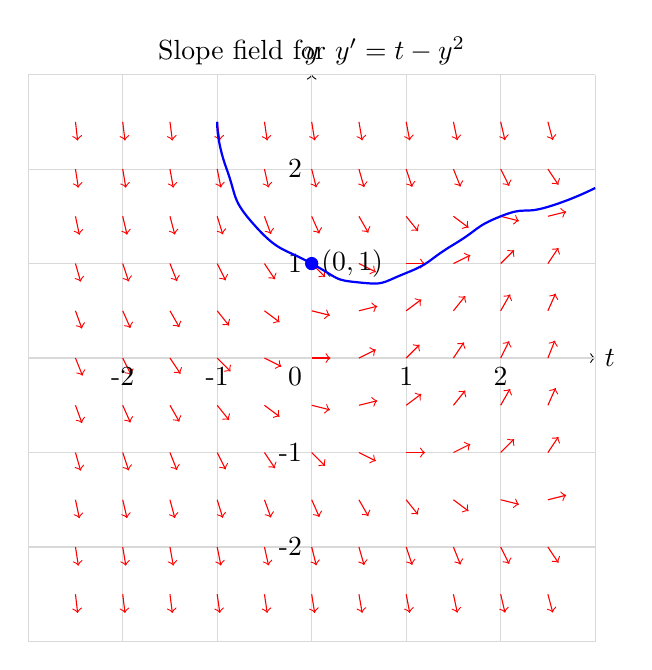
\begin{tikzpicture}[scale=1.2]
        % Draw the axes
        \draw[->] (-3,0) -- (3,0) node[right] {$t$};
        \draw[->] (0,-3) -- (0,3) node[above] {$y$};
        
        % Draw grid lines
        \draw[gray!30] (-3,-3) grid (3,3);
        
        % Draw arrows representing the slope field
        \foreach \x in {-2.5,-2,...,2.5} {
            \foreach \y in {-2.5,-2,...,2.5} {
                \pgfmathsetmacro{\slope}{\x - \y*\y}
                \draw[red,->] (\x,\y) -- ++({0.2*cos(atan(\slope))},{0.2*sin(atan(\slope))});
            }
        }
        
        % Label the axes
        \node[below left] at (0,0) {0};
        \foreach \x in {-2,-1,1,2} {
            \node[below] at (\x,0) {\x};
        }
        \foreach \y in {-2,-1,1,2} {
            \node[left] at (0,\y) {\y};
        }
        
        % Add title
        \node[above] at (0,3) {Slope field for $y' = t - y^2$};
        
        % Mark the initial point
        \fill[blue] (0,1) circle (2pt);
        \node[right] at (0,1) {$(0,1)$};
        
        % Draw the curve following the slope field (corrected direction)
        \draw[thick, blue] plot [smooth, tension=1] 
            coordinates {(-1,2.5) (-0.9,2) (-0.6,1.4) (0,1) (0.5,0.8) (1,0.9) (1.5,1.2) (2,1.5) (2.5,1.6) (3,1.8)};
    \end{tikzpicture}
    \caption{Slope field for $y' = t - y^2$ with initial point $y(0) = 1$ and solution curve}
    \label{fig:slope_field_with_solution_corrected}
\end{figure}















\end{document}
